\chapter{Sprint 0}
\label{Sprint0}
\lhead{Chapter 6. \emph{Sprint 0}}

\section{Goal(s)}
Our first sprint was focused on project planning and preliminary studies.
We wanted to achieve a sufficient understanding of the problem's scope,
relevant technologies and similar solutions as well as complete a high-level planning of
the project which would have included:
\begin{enumerate}[a)]
\item choosing a development process
\item identifying high-level requirements, phases and milestones
\item setting up tools and environments to be used throughout the project.
\end{enumerate}
%\begin{enumerate}[a)]
%\item choosing a development methodology
%\item identifying requirements
%\item identifying phases and milestones
%\item tools to be used
%\end{enumerate}
%Another important goal was to complete a high-level planning of the project
%identifying requirements, phases and milestones; choose a development methodology as well
%as the tools to be used.

\begin{figure}[H]
\centering
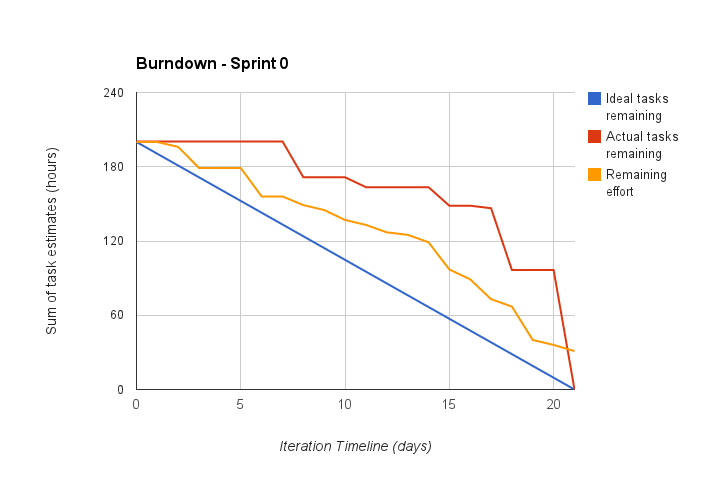
\includegraphics[scale=0.50]{../Figures/burndownSprint0.png}
\caption{Burndown chart Sprint 0}
\label{figure:burndownsprint0}
\end{figure}


\section{Duration}
%This project started on wednesday 21.08.2013 which was the first day of the project and the day we meet the group, the supervisor, the client and got acquainted with the project. We decided early on to use the /ref{Scrum} methodology and to have short sprints so we could focus on some areas at a time. We landed on a total of 6 sprints that each lasted two weeks for a totalt of 12 weeks. Even though we didn't agree on this method before monday the 26th of august we have added the first few days to the first sprint so they also belong in a sprint for tracking the work. Hence the first sprint also includes the first few days of the project making it a total of 13 weeks.
The duration of the sprint was the following:
\begin{itemize}
\item Sprint start: August, 26th
\item Sprint end: September, 8th
\end{itemize}

\section{Planning}

We planned to receive some kind of approval on our understanding of the project
as described by the customer before starting preliminary studies. This was done mainly to avoid
a) planning a solution for a different problem and
b) wasting resources studying something that would not be relevant for the project.
In an effort to prepare a draft of system requirements to be approved by the customer,
%Since the system consists of an integration platform for health data,
we planned some brainstorming sessions to pin down some candidates for health parameters
(weight measurement, blood pressure\ldots) to be supported by the system.
%This would also help us to identify some requirements to submit to the customer.
Additionally, we wanted to decide what software to use to write the report,
choose and setup development enviroments, SDKs and version control systems.

%Because we had to deliver a report for the project, we wanted to decide what software to use to write it.
%Additionally, since we expected to develop at least one Android application
%we planned to setup Android's SDK and development enviroments as well as a version control system.

\section{Backlog}

See below the sprint backlog.
\begin{description}
	\item[Project planning]
		for this sprint included:
		\begin{itemize}
			\item \textbf{Choice of development process}:
				possibile candidates are Waterfall and Scrum.
			\item \textbf{Booking of rooms}:
				where to hold meetings and work.
			\item \textbf{Scheduling weekly meetings}:
				with both the customer and supervisor.
			\item \textbf{Weekly meetings}:
				with both customer and supervisor (starting from September, 26th).
			\item \textbf{Requirements gathering}:
				an initial set (draft) of high-level requirements.
			\item \textbf{Risk analysis}:
				a first draft.
			\item \textbf{Status report}:
				for weeks 35 and 36.
		\end{itemize}
	\item[Preliminary studies]
		of relevant technologies like databases, web-servers and web API.
	\item[Identify possibile data models]
		to be supported by the system (glucose measurement, weight measurement\ldots).
	\item[Choice and setup of project's tools]:
		such as tools for the report and version control system.
	\item[Preliminary system architecture]:
		brainstorm on a high-level architecture to be submitted to the client for feedback.
	\item[Read course's compendium]
	\item[Group dynamics lecture]:
		attendance is mandatory.
	\item[Android environment setup]:
		both IDEs and SDK.
\end{description}


\section{Results and feedback}

\begin{figure}[h]
\centering
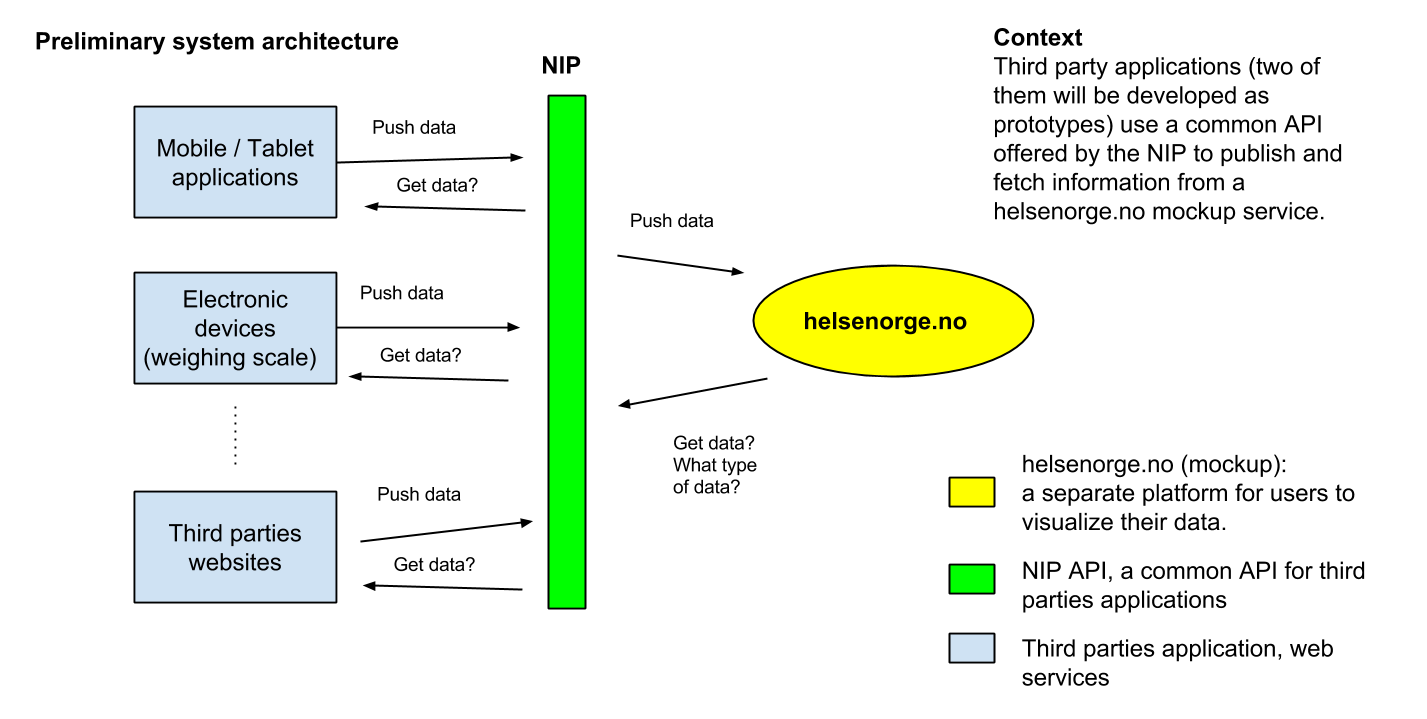
\includegraphics[scale=0.30]{../Figures/architecture-draft.png}
\caption{System architecture (draft)}
\label{figure:architecture-draft}
\end{figure}

During the first days of the project, which were technically not part of any sprint,
we met each other, the customer and the supervisor.
The customer described the problem, explaining what he had in mind and why it was relevant for him.
The supervisor handed us some notes to help the project kick-off.
We exchanged contacts information (both mail and Skype) to make sure everybody could reach out to
everybody else. We set up a Facebook group where to post relevant informations
and a Google Drive folder to share and collaborate on editing documents.
Additionally we scheduled weekly meetings with all involved parties as follows:
\begin{itemize}
\item customer and supervisor meetings on mondays
\item collective work sessions on mondays and wednesdays
\end{itemize}
At the beginning of the sprint we shared our thoughts on what we had understood from the customer.
In order to ensure we had a proper understanding of the problem we produced a diagram
(figure \ref{figure:architecture-draft}) representing a high-level architecture
of the product (an \textit{ehealth integration platform}) as we understood it and submitted
it to the client via mail for feedback.
Having received positive feedback on the proposed system architecture we did some studies
on relevant technologies and searched for similar solutions.
Additionally, we identified a number of candidates for measurement types that were to be supported
by the system and submitted those to the customer as well. We agreed to support heart rate and
weight measurements.
We decided to use Scrum as a development process based on various considerations as
described in \ref{section:development-methodology}. To better perform Scrum, we decided
to use an online tool called \textit{Scrumdo}, described in section \ref{section:tools}.
We also picked and setup other tools like:
\begin{itemize}
\item version control system (Git and GitHub)
\item development environment (IntelliJ IDEA)
\item documentation (LaTeX)
\end{itemize}


%Firstly, the product did not have a clear set of requirements from the beginning and their nature was expected
%to be highly volatile \cite{Sommerville9}. % we expected them to change during the course of the project.
%Secondly, while other process candidates such as Waterfall require a certain degree of expertise,
%Scrum is generally more forgiving. Scrum is also a \textit{lightweight} process, in the sense that introduces
%little overhead compared to other.
%As explained in \ref{ch:studies} Waterfall divides the development cycle in phases \cite{Sommerville9}.
%Each phase has a lot of documentation overhead and appears only once during the project lifetime.
%As such, any failure in any of these phases could have serious consequences on the product.
%On the other hand, Scrum is based on iterations called \textit{sprints}; we figured that iterating the
%same activities each sprint would led our process to eventually improve.

\section{Evaluation}

The sprint generally achieved its expected results.
We achieved a good understanding of the problem and a good overview on high-level system architecture
and requirements. We didn't get as far as we hoped on our studies on some particular technologies and this was
due to a number of factors. Firstly, estimating the amount of time required to obtain a sufficient knowledge
in a topic resulted difficult and we generally needed more time than we thought.
Secondly, we had little familiarity with most involved technologies.
Given the size of our group, we had some difficulties mitigating this problem due to
our reduced technical skill pool. Some difficult topics of study were Apache Camel, its extension Apache IPF,
and if it was desiderable to use these instead of the Spring framework (and why).
Although by the end of the sprint we came to an agreement on what technologies we need to use
(database, web server\ldots) we didn't decide on a specific implementation of such technologies
(Apache Tomcat, Spring, Apache Camel, JAX-RS\ldots).
